\documentclass[fleqn,12pt,letter]{reportY}
\usepackage{microtype}
\usepackage[utf8]{inputenc}
\usepackage[T1]{fontenc}
\usepackage[english]{babel}
\usepackage[left=3.5cm,right=3.5cm,top=2.75cm,bottom=2.75cm]{geometry}
\usepackage{amsmath,amsthm}
\usepackage{xcolor}
\usepackage{fancyhdr}
%\usepackage{amsfonts}
%\usepackage{amssymb}
%\usepackage{}
\usepackage{graphicx}
\numberwithin{figure}{chapter}
\usepackage{graphics,caption,subcaption}
%\usepackage{dsfont}
\usepackage{times}
\usepackage[amsbb]{mtpro2}
\usepackage[colorlinks=false,hidelinks]{hyperref}
\usepackage{csquotes}
\usepackage{multicol}

\usepackage{tikz}
\usetikzlibrary{matrix,shapes,arrows,positioning,chains}
\tikzstyle{decision} = [diamond, draw, fill=blue!20, text width=4.5em, text badly centered, node distance=3cm, inner sep=0pt]
\tikzstyle{block} = [rectangle, draw, fill=white!20, text width=6cm, text centered, rounded corners, minimum height=3em]
\tikzstyle{line} = [draw, -latex']
\tikzstyle{cloud} = [draw, ellipse,fill=red!20, node distance=3cm, minimum height=2em]

\makeatletter
\def\@endtheorem{\endtrivlist}% NEW
\makeatother
\newtheorem{theorem}{Theorem}[chapter]
\newtheorem{corollary}{Corollary}[theorem]
\newtheorem{lemma}[theorem]{Lemma}
\newtheorem{definition}{Definition}[chapter]
\newtheorem{example}{Example}[chapter]

\makeatletter
\def\vect#1{\underline{\sbox\tw@{$#1$}\dp\tw@\z@\box\tw@}}
%\def\tens#1{\mathbf{#1}}
\makeatother


%%%%%%%%%%%%%%%%%%%%%%%%%%%%%%%%%%%%%%%%%%%%%%%%%%%%%%%%%%%%%%%%%%%%%%%%%%%%%
\usepackage{newfloat}
\DeclareFloatingEnvironment[fileext=los,listname=List of Algorithms,name=Algorithm,placement=ht,within=chapter]{algo}
%\usepackage[font={sf,small},labelfont=bf]{caption}
%\captionsetup[figure]{position=above}
\setlength{\intextsep}{15pt plus 3pt minus 2pt}
%\setlength{\floatsep}{5pt plus 3pt minus 2pt}
%\setlength{\textfloatsep}{5pt plus 3pt minus 2pt}
\newsavebox{\coloredbgbox}%
\newenvironment{algobox}%
  {\begin{lrbox}{\coloredbgbox}\begin{minipage}[t]{\textwidth-2\fboxsep-2\fboxrule}\small}%
  {\end{minipage}\end{lrbox}%
   \centering\colorbox{blue!75!black!8}{\usebox{\coloredbgbox}}}%
%%%%%%%%%%%%%%%%%%%%%%%%%%%%%%%%%%%%%%%%%%%%%%%%%%%%%%%%%%%%%%%%%%%%%%%%%%%%%
% fancyhdr parameters
\pagestyle{fancy}
\renewcommand{\chaptermark}[1]{\markboth{\sc\thechapter. #1}{}}
\renewcommand{\sectionmark}[1]{\markright{\thesection\hspace{5pt}#1}{}}
\fancyhf{}
\fancyhead[LE,RO]{\normalfont\normalsize\bfseries\thepage}
\fancyhead[LO]{\rightmark}
\fancyhead[RE]{\leftmark}
\renewcommand{\headrulewidth}{0.5pt}
\addtolength{\headheight}{2.5pt}
\renewcommand{\footrulewidth}{0pt}
\fancypagestyle{plain}{\fancyhead{}\renewcommand{\headrulewidth}{0pt}}
%%%%%%%%%%%%%%%%%%%%%%%%%%%%%%%%%%%%%%%%%%%%%%%%%%%%%%%%%%%%%%%%%%%%%%%%%%%%%
\newcommand*\D{\mathop{}\!\mathrm{d}}
%\newcommand*\diff{\mathop{}\!\mathrm{d}}
\newcommand{\rem}{\textcolor{red}}
\newcommand{\Disp}{\displaystyle}
\newcommand{\expp}{\mathrm{e}}
\newcommand{\vx}{\mathbf{x}}
\newcommand{\vu}{\mathbf{u}}
\newcommand{\vy}{\mathbf{y}}
\newcommand{\vf}{\mathbf{f}}
\newcommand{\mA}{\mathbf{A}}
\newcommand{\fl}{\mathrm{fl}}
\newcommand{\Cont}{\mathcal{C}^0} % C^0 continuity
\newcommand{\ContC}{\mathcal{C}^1} % C^1 continuity
\newcommand{\ContCC}{\mathcal{C}^2} % C^2 continuity
\newcommand{\Contn}{\mathcal{C}^n} % C^n continuity
\newcommand{\base}{\mathsf{b}}
\DeclareMathOperator{\odivide}{\kern.5pt\ominus\kern-9.2pt\div\kern.5pt}
\DeclareMathOperator{\bmax}{\mathbf{max}}
\DeclareMathOperator{\bdiv}{\mathbf{div}}
\DeclareMathOperator*{\argmin}{arg\,min}
%%%%%%%%%%%%%%%%%%%%%%%%%%%%%%%%%%%%%%%%%%%%%%%%%%%%%%%%%%%%%%%%%%%%%%%%%%%%%
\newcommand{\bigO}{O} % big O
%\newcommand{\bigO}{\mathscr{O}} % big O
%\newcommand{\nsubset}{\not\subset}
%%%%%%%%%%%%%%%%%%%%%%%%%%%%%%%%%%%%%%%%%%%%%%%%%%%%%%%%%%%%%%%%%%%%%%%%%%%%%
\newcommand{\inteoo}[2]{\mathopen{(}#1\,;#2\mathclose{)}}
\newcommand{\inteff}[2]{\mathopen{[}#1\,;#2\mathclose{]}}
\newcommand{\inteof}[2]{\mathopen{(}#1\,;#2\mathclose{]}}
\newcommand{\intefo}[2]{\mathopen{[}#1\,;#2\mathclose{)}}
\newcommand{\intg}[2]{\mathopen{(}#1\,;#2\mathclose{)}}
%%%%%%%%%%%%%%%%%%%%%%%%%%%%%%%%%%%%%%%%%%%%%%%%%%%%%%%%%%%%%%%%%%%%%%%%%%%%%
\usepackage{listings}
\definecolor{mygreen}{RGB}{28,172,0} % color values Red, Green, Blue
\definecolor{mylilas}{RGB}{170,55,241}

\definecolor{mycolor1}{rgb}{0.00000,0.44700,0.74100}%
\definecolor{mycolor2}{rgb}{0.85000,0.32500,0.09800}%
\definecolor{mycolor4}{rgb}{0.49400,0.18400,0.55600}%
\definecolor{mycolor3}{rgb}{0.9290    ,0.6940    ,0.1250}
\DeclareRobustCommand{\colorlineA}{\tikz[baseline=-\the\dimexpr\fontdimen22\textfont2\relax,inner sep=0pt]\draw[mycolor1,solid,line width=1pt](0,0) -- (5mm,0);}
\DeclareRobustCommand{\colorlineB}{\tikz[baseline=-\the\dimexpr\fontdimen22\textfont2\relax,inner sep=0pt]\draw[mycolor2,solid,line width=1pt](0,0) -- (5mm,0);}
\DeclareRobustCommand{\colorlineC}{\tikz[baseline=-\the\dimexpr\fontdimen22\textfont2\relax,inner sep=0pt]\draw[mycolor3,solid,line width=1pt](0,0) -- (5mm,0);}
\DeclareRobustCommand{\colorADashed}{\tikz[baseline=-\the\dimexpr\fontdimen22\textfont2\relax,inner sep=0pt]\draw[mycolor1,dashed,line width=1pt](0,0) -- (5mm,0);}
\DeclareRobustCommand{\colorBDashed}{\tikz[baseline=-\the\dimexpr\fontdimen22\textfont2\relax,inner sep=0pt]\draw[mycolor2,dashed,line width=1pt](0,0) -- (5mm,0);}
\DeclareRobustCommand{\colorCDashed}{\tikz[baseline=-\the\dimexpr\fontdimen22\textfont2\relax,inner sep=0pt]\draw[mycolor3,dashed,line width=1pt](0,0) -- (5mm,0);}
\DeclareRobustCommand{\colorDDashed}{\tikz[baseline=-\the\dimexpr\fontdimen22\textfont2\relax,inner sep=0pt]\draw[mycolor4,dashed,line width=1pt](0,0) -- (5mm,0);}
\DeclareRobustCommand{\blackSolid}{\tikz[baseline=-\the\dimexpr\fontdimen22\textfont2\relax,inner sep=0pt]\draw[black,solid,line width=1pt](0,0) -- (5mm,0);}
\DeclareRobustCommand{\blackDashed}{\tikz[baseline=-\the\dimexpr\fontdimen22\textfont2\relax,inner sep=0pt]\draw[black,dashed,line width=1pt](0,0) -- (5mm,0);}
\DeclareRobustCommand{\blackDashdotted}{\tikz[baseline=-\the\dimexpr\fontdimen22\textfont2\relax,inner sep=0pt]\draw[black,dashdotted,line width=1pt](0,0) -- (5mm,0);}
\DeclareRobustCommand{\colorlineDashedBlack}{\tikz[baseline=-\the\dimexpr\fontdimen22\textfont2\relax,inner sep=0pt]\draw[black,dashed,line width=1pt](0,0) -- (5mm,0);}
\DeclareRobustCommand{\colorlineBDashed}{\tikz[baseline=-\the\dimexpr\fontdimen22\textfont2\relax,inner sep=0pt]\draw[mycolor2,dashed,line width=1pt](0,0) -- (5mm,0);}


\lstset{language=matlab,%
    %%%%%%%%%%%%%%%%%%%basicstyle=\color{red},
    breaklines=true,%
    morekeywords={matlab2tikz},
    keywordstyle=\color{blue},%
    morekeywords=[2]{1}, keywordstyle=[2]{\color{black}},
    identifierstyle=\color{black},%
    stringstyle=\color{mylilas},
    commentstyle=\color{mygreen},%
    showstringspaces=false,%without this there will be a symbol in the places where there is a space
    numbers=left,%
    numberstyle={\tiny \color{black}},% size of the numbers
    numbersep=9pt, % this defines how far the numbers are from the text
    %emph=[1]{for,end,break},emphstyle=[1]\color{red}, %some words to emphasise
    %%%%%%%%%%%%%%%emph=[2]{word1,word2}, emphstyle=[2]{style}, 
    flexiblecolumns=true,
	stringstyle=\ttfamily\footnotesize, % typewriter type for strings
	basicstyle=\ttfamily\footnotesize, % typewriter type for strings
	frame=single,
	backgroundcolor=\color{blue!75!black!8},
	rulecolor=\color{blue!50},
	framesep=0pt,
	rulesep=0pt,
	framerule=0pt,
	framexleftmargin=0pt,
}


\usepackage{algorithmic}
\usepackage{eqparbox}
%\renewcommand{\algorithmiccomment}[1]{\hfill\eqparbox{COMMENT}{$\triangleright$\ #1}}
\renewcommand\algorithmiccomment[1]{\hfill$\triangleright$\ \eqparbox{COMMENT}{#1}}%

\newcommand{\B}[1]{\mathbf{#1}}
\newcommand{\cmm}[1]{\textcolor{red}{#1}}


\definecolor{codegreen}{rgb}{0,0.6,0}
\definecolor{codegray}{rgb}{0.5,0.5,0.5}
\definecolor{codeamber}{rgb}{1,.49,0}
\definecolor{backcolour}{rgb}{0.95,0.95,0.92}
 
% Default fixed font does not support bold face
\DeclareFixedFont{\ttb}{T1}{txtt}{bx}{n}{9} % for bold
\DeclareFixedFont{\ttm}{T1}{txtt}{m}{n}{9}  % for normal
\lstdefinestyle{mystyle}{
    backgroundcolor=\color{backcolour},   
    commentstyle=\color{red},
    keywordstyle=\color{codeamber},
    numberstyle=\tiny\color{codegray},
    stringstyle=\color{codegreen},
    basicstyle=\linespread{1.1}\footnotesize\ttm,
    breakatwhitespace=false,         
    breaklines=true,                 
    captionpos=b,                    
    keepspaces=true,                 
    numbers=left,                    
    numbersep=5pt,                  
    showspaces=false,                
    showstringspaces=false,
    showtabs=false,                  
    tabsize=2}
 
\lstset{style=mystyle}

\bibliographystyle{apalike}\title{User manual}
\author{Yulin Shi \\ \href{http://structdynviblab.mcgill.ca/}{Structural dynamics and vibration laboratory} \\ McGill University }
\begin{document}
\maketitle
%% ------------------------------------------- -------------------------------------------
\chapter{Static contact problem}
%% ------------------------------------------- -------------------------------------------
\section{Semismooth Newton method}
\begin{algo}
\begin{algobox}
\begin{algorithmic}[1]
\STATE \textbf{Input}: Semismooth function $\vf(\vx): \mathbb R^N \rightarrow \mathbb R^N$ and initial guess $\vx\in \mathbb R^N$; tolerance $\varepsilon>0$ 
\STATE \textbf{Init}: Initial guess $\vx\in \mathbb R^N$ 
\WHILE {Norm of residual $\Vert \vf(\vx) \Vert > \varepsilon$}
	\STATE Calculate the residual $\vf(\vx)$
	\STATE Select a Jacobian matrix $\mathbf G(\vx)$ in the sub-differential set $\partial \vf(\vx)$
	\STATE Update $\vx \leftarrow \vx - \mathbf G(\vx)^{-1} \vf(\vx)$
\ENDWHILE
\end{algorithmic}
\end{algobox}
\caption{Semismooth Newton method \cite{hintermuller2010semismooth,fischer1992special}.}\label{al:static/semismooth}
\end{algo}
%% ------------------------------------------- -------------------------------------------
\section{One degree-of-freedom contact problem}
\begin{figure}[ht]
\centering
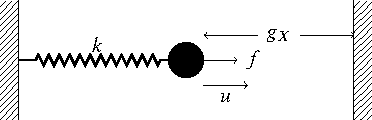
\includegraphics[scale=1]{figure/mass_spring_one_dof/tikz}
\caption{One degree-of-freedom contact problem $ku=\lambda +f$ and $u\leq g_X$ where $u$ is the displacement, $\lambda$ is the contact force, $k$ is the stiffness, $f$ is the external force and $g_X$ is the initial gap. Define the normal gap as $g_N(u)=u-g_X$, denote the penetration as $g_N^+$}
\label{mass_spring_one_dof}
\end{figure}
%% ------------------------------------------- -------------------------------------------
\section{Semismooth reformulation}
\begin{equation}
\begin{cases}
r(u,\lambda ) = ku-\lambda -f = 0
\\	s(u,\lambda) = \lambda + \max \{ 0, c(u-g_X) - \lambda \} =0 
\end{cases}
\end{equation}
where positive constant $c$ is used to balance the unit between displacement and force. Function $s(u,\lambda): \mathbb R^2 \rightarrow \mathbb R $ is semismooth. Solve it with semismooth Newton method.
%% ------------------------------------------- -------------------------------------------
\section{Penalty treatment}
Regularize the non-differentiable contact constitutive law using a constant penalty coefficient $\epsilon$ as is reviewed in \cite{wriggers2006computational} 
\begin{equation}\label{eq:static/penalty11}
\lambda(u) = -\epsilon \max\{ 0, u-g_X\}
\end{equation}
And get the regularized system equation to be solved: 
\begin{equation}\label{eq:static/penalty12}
r(u) = ku-\lambda(u) -f = 0
\end{equation}
where positive constant $c$ is used to balance the unit between displacement and force. Function $r(u): \mathbb R \rightarrow \mathbb R $ is semismooth. 

The solution of the regularized system converges to true solution when $\epsilon \rightarrow \infty$. It yields the algorithm \ref{al:penalty_finite} 
\begin{algo}
\begin{algobox}
\begin{algorithmic}[1]%
\STATE \textbf{Input}: coefficient matrices $\mathbf K$, $\vf$ and $\mathbf G$ (linear or nonlinear w.r.t. $\mathbf u$), penalty coefficient $\epsilon$ and error tolerances $\varepsilon$ and $\varepsilon_1$.
\STATE \textbf{Initialization}: $\mathbf u$. 
\WHILE { $|| \Delta \mathbf u|| > \varepsilon $ }
	\STATE Increase $\epsilon$
	\WHILE { $|| \Delta \mathbf u || > \varepsilon_1 $ }
		\STATE Solve \eqref{eq:static/penalty12} using semismooth Newton method in algorithm \ref{al:semismooth}
	\ENDWHILE
\ENDWHILE
\end{algorithmic}
\end{algobox}
\caption{Solve finite contact problem in penalty form by semismooth Newton method.}\label{al:penalty_finite}
\end{algo}
%% ------------------------------------------- -------------------------------------------
\section{Augmented Lagrange treatment and Uzawa algorithm}
In augmented Lagrange method, the contact force is the sum of a constant term and the penalty term with small $\epsilon$ as is reviewed in \cite{wriggers2006computational}
\begin{equation}\label{eq:static/augmented11}
\lambda(u) = \bar{\lambda} - \epsilon \max\{ 0, u-g_X\}
\end{equation}
And get the regularized system equation to be solved: 
\begin{equation}\label{eq:static/augmented12}
r(u) = ku-\lambda(u) -f = 0
\end{equation}
where positive constant $c$ is used to balance the unit between displacement and force. Function $r(u): \mathbb R \rightarrow \mathbb R $ is semismooth. 

The augmented term $\bar{p}_N$ is fixed within an iteration step, as to preserve the contact stress. It is updated as 
\begin{equation}\label{eq:aug_lagrange_update}
\bar{\lambda}= \min \{ 0, \bar{\lambda} - \epsilon \max\{ 0, u-g_X\} \}
\end{equation}

It yields a double-loop algorithm. In the inner loop, solve the nonlinear equation with fixed augmented term $\bar{\lambda}$ and fixed penalty coefficient $\epsilon$, in the outer loop, update these two coefficients. An empirical updating law of $\epsilon$ given by \cite{bertsekas2014constrained}
\begin{equation}\label{eq:aug_penalty_update_bertsekas}
\epsilon \leftarrow
10\epsilon
,\\
||g_N^{+,(k+1)}|| > \frac{1}{4} ||g_N^{+,(k)}|| 
\end{equation}

\begin{algo}
\begin{algobox}
\begin{algorithmic}[1]%
\STATE \textbf{Input}: coefficient matrices of the discretized problem \eqref{eq:penalty_finite} and error tolerances $\varepsilon$ and $\varepsilon_1$.
\STATE \textbf{Initialization}: $u, \bar{\lambda}, \epsilon$. 
\WHILE { $|| r(u) || > \varepsilon $ }
	\WHILE { $|| r(u)|| > \varepsilon_1 $ }
		\STATE Solve \eqref{eq:static/augmented12} using semismooth Newton method in algorithm \ref{al:semismooth}
	\ENDWHILE
	\STATE update $ \bar{\lambda}$ according to \eqref{eq:aug_lagrange_update} 
	\STATE update $\epsilon$ according to \eqref{eq:aug_penalty_update_bertsekas}
\ENDWHILE
\end{algorithmic}
\end{algobox}
\caption{Penalty method for finite contact problem}\label{al:static/augmented}
\end{algo}

\end{document}